%!TEX root = report.tex
\section{Robot movement}

\subsection{Control}

The movement of the robot is controlled via two 150W DC motors of nominal current 5.77 A. Each motor has an incremental encoder with 512 pulses per revolution. Given the gear ratio of 43:1, this leads to a total number of pulses per revolution of $N_{tot}=22016$.
The robot is two-wheeled with a third, passive swivel wheel for stabilization.
It comes with a already implemented control software with 3 control modes that may be chosen from: position control, speed control and speed/acceleration control. 
For the present setup, speed/acceleration mode is used since the robot shall be moved at a certain speed but its acceleration should be limited to avoid abrupt movements. (see Figure \ref{fig:acceleration})
Position control was considered but the high amount of user input required for good functioning made it undesirable compared to speed/acceleration control.

\begin{figure}[htb]
    \centering
    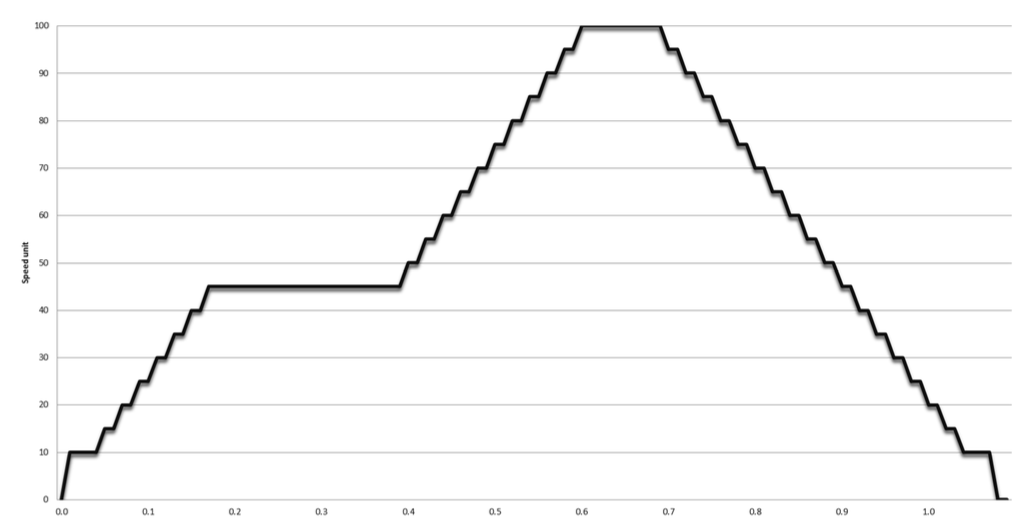
\includegraphics[width=0.5\linewidth]{files/Acceleration.png}
    \caption{Speed profile for acceleration from 0 to 45, followed by 45 to 100 and a deceleration down to 0 in speed/acceleration control mode}
    \label{fig:acceleration}
\end{figure}

\subsection{Odometry}

\begin{figure}[htb]
    \centering
    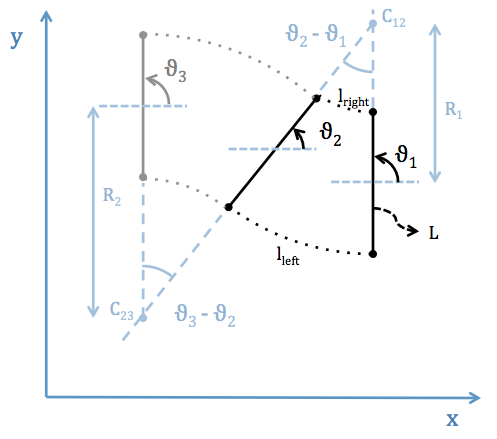
\includegraphics[width=0.5\linewidth]{files/Odometry.png}
    \caption{Geometry consdierations for odometry}
    \label{fig:odometry}
\end{figure}

The following considerations follow from basic geometry and \cite{Borenstein1996}.
Given the incremental encoder readings from the left and the right motor respectively ($e_{left,i},e_{right,i}$) and assuming no slip of the wheels on the ground, odometry allows to calculate the relative change in position as follows.
First of all, the odometry measurements can be converted in the trajectory length using
\begin{align}
    l_{left,i} &= \frac{2\pi R_{wheels} e_{left,i}}{N_{tot}} \\
    l_{right,i} &= \frac{-2\pi R_{wheels} e_{right,i}}{N_{tot}}
    \label{eq:encoders} 
\end{align}
Note that the right encoder reading is inverted because of the mounting of the wheels facing in opposite directions.
Starting from a first position $\begin{bmatrix} x_i,y_i,\theta_i \end{bmatrix}$, where $\theta_i$ denotes the rotation with respect to the x axis, the next position is obtained with the following formulas:

\begin{subequations}
    \begin{align}
        \theta_{i+1} &= \theta_i + \frac{l_{left,i}-l_{right,i}}{L} \\
        y_{i+1} &= y_i + |R_i| (\cos(\theta_{i+1}-\theta_{i})-1) \\
        x_{i+1} &= x_i + R_i \sin(\theta_{i+1}-\theta_i) \\
        \text{where} \quad R_{i+1} &= \frac{L}{2} \frac{l_{left,i}+l_{right,i}}{l_{left,i}-l_{right,i}} 
    \label{eq:positions}
\end{align}
\end{subequations}

$L$ is length of the robot axis or the distance between the two wheels. 
$R$ denotes the radius of the circle formed by the center of the robot axis with center $C_{i,i+1}$ (see Figure \ref{fig:odometry}).

\subsection{Experimental Results}

%\begin{lstlisting}[caption=Listing]
%\end{lstlisting}

%\begin{figure}[htb]
%	\centering
%	\begin{subfigure}[b]{0.49\linewidth}
%		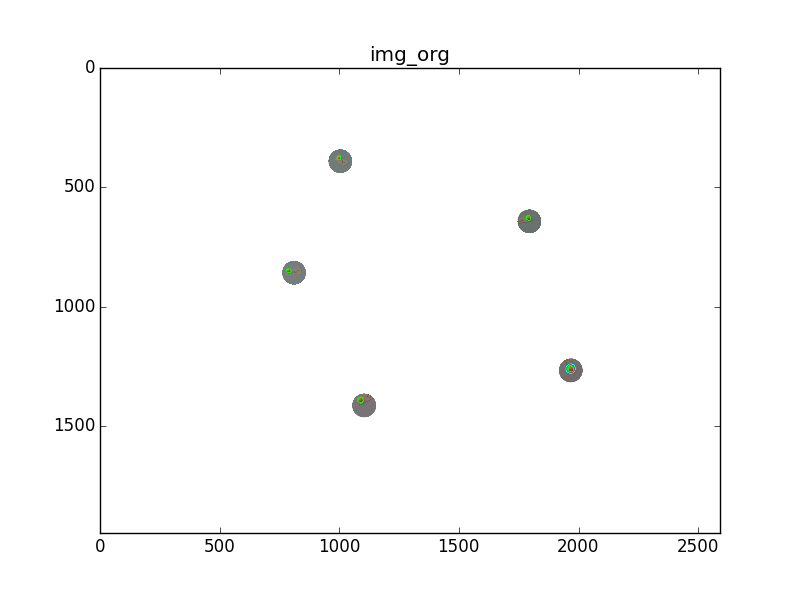
\includegraphics[width=\linewidth]{../files/img_org139.png}
%		\caption{Regions of interest chosen by user and extracted colors}
%		\label{feat_step0}
%	\end{subfigure}
%	\begin{subfigure}[b]{0.49\linewidth}
%		\includegraphics[width=\linewidth]{../files/img_h139.png}
%		\caption{\textit{Hue} representation of original image}
%		\label{feat_step1}
%	\end{subfigure}
%	\begin{subfigure}[b]{0.49\linewidth}
%		\includegraphics[width=\linewidth]{../files/img_s139.png}
%		\caption{\textit{Saturation} representation of original image}
%		\label{feat_step2}
%	\end{subfigure}
%	\begin{subfigure}[b]{0.49\linewidth}
%		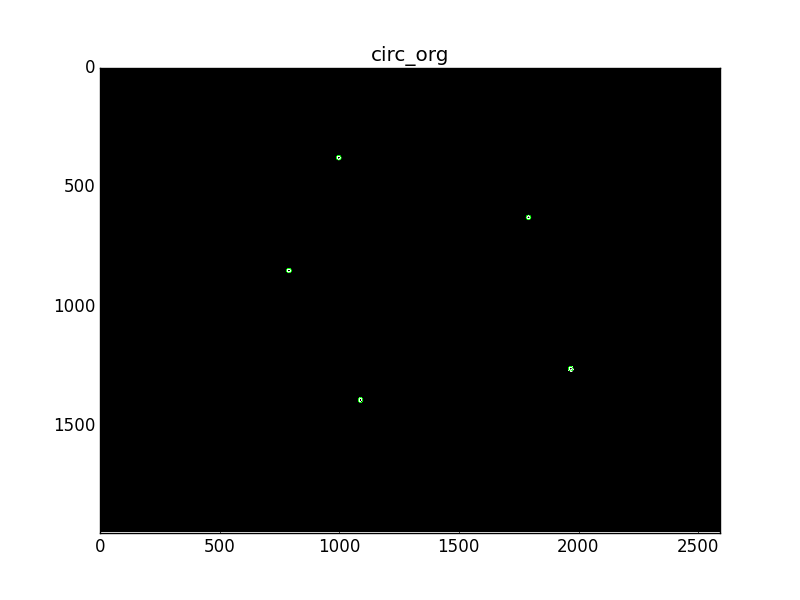
\includegraphics[width=\linewidth]{../files/circ_org139.png}
%		\caption{Regions of interest chosen by user and extracted colors}
%		\label{feat_step3}
%	\end{subfigure}
%	
%	
%	\begin{subfigure}[b]{0.49\linewidth}
%		\includegraphics[width=\linewidth]{../files/zdot_RefTrackNL.png}
%	\end{subfigure}
%	\begin{subfigure}[b]{0.49\linewidth}
%		\includegraphics[width=\linewidth]{../files/speeds_RefTrackNL.png}
%	\end{subfigure}
%	\begin{subfigure}[b]{0.49\linewidth}
%		\includegraphics[width=\linewidth]{../files/xyz_RefTrackNL.png}
%	\end{subfigure}
%	\caption{Procedure for feature extraction} 
%\end{figure}
